%% A simple template for a term report using the Hagenberg setup 
%% based on the standard LaTeX 'report' class

%%% Magic comments for setting the correct parameters in compatible IDEs
% !TeX encoding = utf8
% !TeX program = pdflatex 
% !TeX spellcheck = en_US
% !BIB program = biber

\RequirePackage[utf8]{inputenc} % Remove when using lualatex or xelatex!
\RequirePackage{hgbpdfa}        % Creates a PDF/A-2b compliant document

\documentclass[english,notitlepage,smartquotes]{hgbreport}
% Supported options in [..]:
%    Main language: 'german' (default), 'english'
%    Conversion to typographic quotation marks: 'smartquotes'
%    Use APA citation style: 'apa'
%    Do not create a separate title page: 'notitlepage'
%    Page layout: 'oneside' (single-sided, default), 'twoside' (double-sided)
%%%-----------------------------------------------------------------------------

\graphicspath{{images/}}  % Location of images and graphics
\bibliography{references} % Biblatex bibliography file (references.bib)
% theorems, definitions, remarks etc.
\usepackage{amsthm}

\theoremstyle{definition}
\newtheorem{definition}{Definition}

\theoremstyle{definition}
\newtheorem{problem}{Problem}

\theoremstyle{remark}
\newtheorem*{remark}{Remark}

\theoremstyle{plain}
\newtheorem{theorem}{Theorem}[chapter]
\newtheorem{corollary}{Corollary}[theorem]
\newtheorem{lemma}{Lemma}[chapter]
\newtheorem{mini-theorem}{Mini-theorem}
\theoremstyle{definition}
\newtheorem{example}{Example}
\renewcommand\qedsymbol{$\blacksquare$}
% theorems, definitions, remarks etc.
% the "reflection" box
\usepackage[framemethod=tikz]{mdframed}
\theoremstyle{definition}
\newtheorem{reflection}{Reflection}
\mdfdefinestyle{reflectionbox}{
  innertopmargin=\topskip,
  roundcorner=5pt,
  linecolor=cyan,
  backgroundcolor=cyan!20,
}
\surroundwithmdframed[style=reflectionbox]{reflection}
% the "reflection" box

% long table
\usepackage{longtable}
% long table

% for algorithm description
\usepackage{algorithm}
\usepackage{algpseudocodex}
% for algorithm description
% for images etc.
\usepackage{tikz}
\newcommand*\circled[1]{\tikz[baseline=(char.base)]{
    \node[shape=circle,draw=red,inner sep=2pt] (char) {#1};}}
\newcommand*\fillcircled[2]{\tikz[baseline=(char.base)]{
    \node[shape=circle,fill=#2,draw=red,inner sep=2pt] (char) {#1};}}
% for images etc.
% color names
\usepackage[dvipsnames]{xcolor}
% color names
% Big starting letters
\usepackage{lettrine}
% Big starting letters
% cancel terms
\usepackage{cancel}
% cancel terms

% sidebar environment https://tex.stackexchange.com/a/735167/64425
\usepackage[most]{tcolorbox}

\newtcolorbox{sidebar}{
  breakable,
  enhanced,
  frame hidden,
  interior hidden,
  size=minimal,
  left skip=8pt,
  borderline west={1pt}{-5pt}{gray}
}
% sidebar environment https://tex.stackexchange.com/a/735167/64425

% 
\usepackage{parskip}% http://ctan.org/pkg/parskip
%
% get rid of ugly borders
\hypersetup{
    colorlinks,
    linkcolor={magenta!50!black},
    citecolor={blue!50!black},
    urlcolor={blue!80!black}
}
% get rid of ugly borders

% some commands, mainly for local use
% some commands, mainly for local use
%%%-----------------------------------------------------------------------------
\begin{document}
%%%-----------------------------------------------------------------------------
\author{Kedar Mhaswade}                    % Your name
\title{Linear Algebra Problem Book:\\ % Name of the course or project
			Notes and Problem Solutions}	                 % or "Project Report"
\date{04 June 2025}

%%%-----------------------------------------------------------------------------
\maketitle
%%%-----------------------------------------------------------------------------
\begin{abstract}\noindent

\bigskip
\noindent
% Use the abstract to provide a short summary of the document's contents.
\lettrine[lines=3]{T}{his} is an objective, yet personal, narrative of the author's odyssey in the enchanted land of linear algebra. It contains his notes and solutions to problems from Professor Paul Halmos's \cite{Halmos1995} \textit{Linear Algebra Problem Book}.


I like to write. I don't have an established audience, but that does not deter me from writing. However, I have often wondered why I should carefully typeset my mathematical writing using a comprehensive system like \LaTeX. First, my mathematical writing is not `research' yet, but mainly problem-solving (which does involve at least some dogged pursuit, if not research). Second, I love writing by hand! 
\begin{figure}[!h]
\begin{center}
\caption{Handwriting is fun!}
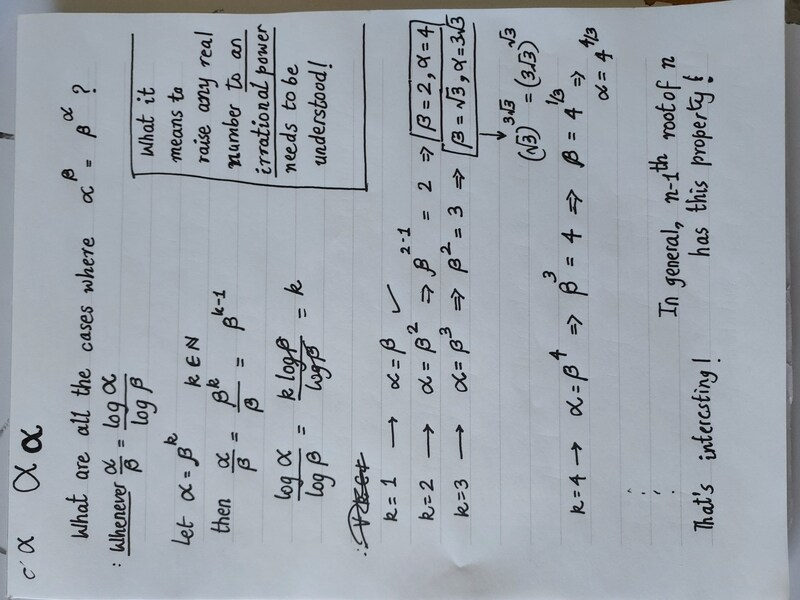
\includegraphics[width=.345\textwidth,angle=-90]{loving-to-write-by-hand-small}
\end{center}
\end{figure}

Freehand writing on a good paper with a good pen is fun. It's quick. It's rewarding.

Typesetting is, on the other hand, time-consuming and feels like \textit{Yak-shaving} \cite{Yak-shaving}. However, all good life is controlled Yak-shaving. When I typeset {\LaTeX} documents, I tend to minimize Yak-shaving and focus on having a conversation with myself. I suspect that I understand the subject matter better that way. I like the following quote in this regard:

\begin{sidebar}
I don't know what I think unless I read what I write. --Unknown
\end{sidebar}

Of course, you cannot begin solving problems on a computer. A pencil and papers are must. In this respect, typesetting is favoring form over content. We strive to present beautifully what we have thought well but scribbled hastily. Fortunately, I don't mind taking the time to do that; it at least keeps me busy fine-tuning my thoughts. It sometimes even helps to find flaws.

However, the biggest advantage of typesetting my writing is keeping a record of beautifully typeset account of something, anything. If I could ever make a case to study under a stalwart like Professor Yaser Abu-Mostafa (\url{https://work.caltech.edu/}), or Professor Avrim Blum (\url{https://home.ttic.edu/~avrim/}), perhaps I can demonstrate what I have done in my scarce free time.

I have gone back and forth between handwritten pages and typeset manuscripts. However, I am resorting to typesetting for this work despite the overhead incurred. I hope I follow through. It's one thing to be motivated but another to be determined and disciplined.

Perhaps a picture (Figure [\ref{fig:mindmap}]) can explain better than words how I started reading Halmos's book. 

\begin{figure}[!h]
\begin{center}
\caption{A June 2025 Mindmap}
\label{fig:mindmap}
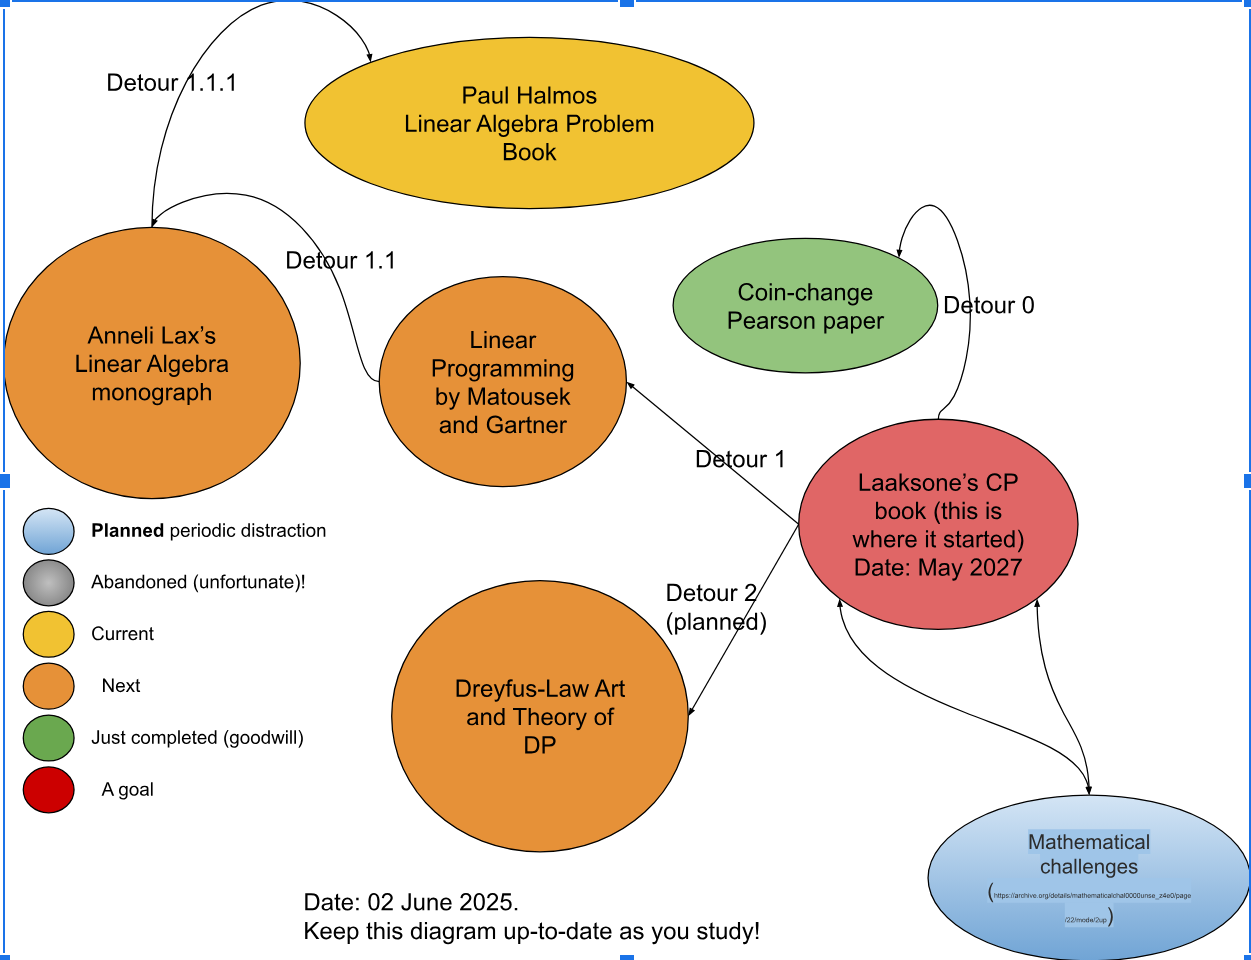
\includegraphics[width=.5\textwidth]{june-2025-mindmap}
\end{center}
\end{figure}

I will avoid answering ``Why Halmos's Linear Algebra book?'' It suffices to say that his style resonates with me, a teaser of which can be enjoyed from what follows:

\begin{sidebar}
Is it obvious that
$$ 63+48=27+84$$?
It is a true and thoroughly uninteresting mathematical statement that can be verified in a few seconds--but is it \textit{obvious}? If calling it obvious means that the reason for its truth is clearly understood, without even a single second's verification, then most people would probably say no.

What about
$$ (27+36)+48=27+(36+84)$$
?
--is that obvious?
Yes it is, for most people; the instinctive (and correct) reaction is that the way the terms of a sum are bunched together cannot affect the answer. The approved technical term is not ``bunch together'' but ``associate''; the instinctive reaction is a readiness to accept what is called the \textbf{associative law} of addition for real numbers. (Surely every reader has noticed by now that the non-obvious statement and the obvious one are in some sense the same:

$$ 63=27+36\quad and\quad 84=36+48$$)

\textbf{Linear algebra is concerned with several different kinds of operations (such as addition) on several different kinds of objects (not necessarily real numbers)}. To prepare the ground for the study of strange operations and to keep the associative law from being unjustly dismissed as a triviality, a little effort to consider some good examples and some bad ones is worthwhile.

Some of the examples will be useful in the sequel, and some won't--some are here to show that associativity can fail, and others are here to show that even when it holds it may be far from obvious. In the world of linear algebra non-associative operations are rare, but associative operations whose good behavior is not obvious are more frequently met.

\end{sidebar}

Paul Halmos has been one of my favorite authors. His insistence on problem-solving is admirable. I hope I can painstakingly (and gleefully at the same time) solve a number of problems from this book, and understand at least some of linear algebra. The problems have been solved by Halmos himself and the answers appear at the back of this book (Thank You!), but these solutions are mine. I have also felt free to think aloud, write willfully about questions that came to my mind as I solved the stated problems. That part of writing appears like `personal reflections':
\begin{reflection}
Problems come in various levels of difficulty. And, unless you are George Dantzig (who solved an open problem written on a blackboard assuming his instructor had given a homework assignment) or the like, you have to toil through them. Some you are able to solve quickly, perhaps because you are experiencing ``flow''\footnote{A highly focused mental state, defined and popularized by the psychologist Mihaly Csikszentmihalyi, conducive to productivity}, but many are challenging and you suffer (albeit purposefully) through them. They are distinct from exercises, which are also essential for fluency and emotional well-being, but expected to be aimed at `practice' and easier to answer.
\end{reflection}
Feel free to skip them. As Halmos urges us in his preface to this book, I have read his solutions too. He considers solutions an integral part of exposition. The $\blacksquare$ (the QED symbol) appears after every solution. Wherever desired, I have also reinterpreted Halmos's solutions; understanding them will be certainly helpful. He has also provided hints first: Definitions, theorems, and problems, followed by hints for each problem, followed by complete solutions. There aren't very many authors who work so hard on their book!

Readable and flawless mathematical typesetting is hard. It's ironic that the epitome of exact sciences breeds a degree of inexactness in notation. Like in literature, meaning sometimes depends on context not captured in notation. And yet, an encyclopedic treatment of notation at the beginning of a work like this tends to bore readers\footnote{What disappointments them even more are typos and errors.}. Here too, a balance needs to be sought. A few conventions are therefore in order:

\begin{itemize}
\item A roman letter in italics, like, for example, $p$, generally denotes a real number, unless specified otherwise (sometimes an integer). This is different from a number theory convention. 
\item Greek letters usually denote real numbers.
\item The so-called \verb|\cdot|: $\cdot$ to denote multiplication is sometimes omitted. Thus, $ab$ is equivalent (and often even preferred and ubiquitous, thanks to Euler!) to $a\cdot b$.

\end{itemize}
\end{abstract}

%%%-----------------------------------------------------------------------------
\tableofcontents
%%%-----------------------------------------------------------------------------

%%%-----------------------------------------------------------------------------
\chapter{Scalars}
%%%-----------------------------------------------------------------------------
\begin{problem}
\label{pr:2a2b}
If a new addition for real numbers, denoted by the temporary symbol $\boxplus$, is defined by
$$
\alpha\boxplus\beta=2\alpha+2\beta
$$
, is $\boxplus$ associative?

Note: The $+$ sign on the right denotes ordinary addition.

Note: The new operation $\boxplus$ is \textit{commutative}: $\alpha\boxplus\beta=2\alpha+2\beta$ indeed equals $\beta\boxplus\alpha=2\beta+2\alpha$.
\end{problem}

\textbf{Solution}.

No. We can easily demonstrate 

$$
\alpha\boxplus(\beta\boxplus\gamma)\ne(\alpha\boxplus\beta)\boxplus\gamma
$$


\qedsymbol

\begin{problem}
\label{pr:2ab}
If a new addition for real numbers, denoted by the temporary symbol $\boxplus$, is defined by
$$
\alpha\boxplus\beta=2\alpha+\beta
$$
, is $\boxplus$ associative?
\end{problem}

\textbf{Solution}.

No. We can easily demonstrate 

$$
\alpha\boxplus(\beta\boxplus\gamma)\ne(\alpha\boxplus\beta)\boxplus\gamma
$$
\qedsymbol

\begin{problem}
\label{pr:atob}
If an operation for \emph{positive integers}, denoted by the temporary symbol $*$, is defined by
$$
\alpha*\beta=\alpha^\beta
$$
, is it commutative? Is it associative?
\end{problem}

\textbf{Solution}.

Although $\alpha^\beta=\beta^\alpha$ when $\alpha=\beta$, in general, $\alpha^{\beta}$ doesn't seem to equal $\beta^\alpha$. A simple counterexample is $\alpha=1,\beta=2$. Therefore, $*$ is not a commutative operation on two positive integers.
\qedsymbol

\begin{reflection}

I asked myself, ``For which real numbers $\alpha,\beta$ (although in Problem [\ref{pr:atob}] they are positive integers) are $\alpha^\beta$ and $\beta^\alpha$ equal?''

The following exploration amazed me.
$$
\alpha^\beta=\beta^\alpha
$$
\begin{equation}
\label{eq:takelogs}
\therefore \beta\log\alpha=\alpha\log\beta
\end{equation}

\begin{equation}
\label{eq:ablogalob}
\therefore \frac{\alpha}{\beta}=\frac{\log\alpha}{\log\beta}
\end{equation}

A general solution of equation [\ref{eq:ablogalob}] (a Diophantine equation for we seek integer solutions) is perhaps hard, but somehow I asked, ``What if $\alpha=\beta^k$ for some $k\in\mathbb N$?'' I don't know why I thought of that. Is that intuition? Maybe.

Equation [\ref{eq:ablogalob}] then gives
$$
\frac{\beta^k}{\beta}=\frac{k\cancel{\log\beta}}{\cancel{\log\beta}}
$$
which simplifies to

\begin{equation}
\label{eq:bk-1k}
\beta^{k-1}=k
\end{equation}


%\begin{table}[h!]
%\centering
\begin{tabular}{|c|c|c|}
 \hline
 $k$ & What follows from $\alpha=\beta^k$ & $\alpha,\beta$ \\ \hline
 \hline
 $1$ & $\alpha=\beta$  & Any real numbers \\ \hline
 $2$ & $\beta^{2-1}=\beta=2$ & $\alpha=4,\beta=2$ \\ \hline
 $3$ & $\beta^{3-1}=\beta^2=3$ & $\alpha=3\sqrt{3},\beta=\sqrt{3}$ \\ \hline
 $4$ & $\beta^{4-1}=\beta^3=4$ & $\alpha=4\sqrt[3]{4},\beta=\sqrt[3]{4}$ \\ \hline
\end{tabular}

%\caption{When does $\alpha^\beta=\beta^\alpha$ if $\alpha=\beta^k, k\in\mathbb N$?}
%\label{tab:ab=ba}
%\end{table}

That was interesting! 

\end{reflection}

Exponentiation is associative only when $\beta\gamma=\beta^\gamma$. There are specific cases when that is true (e.g. $\beta=\gamma=2$), but it is not true in general. A simple counterexample is $\alpha=2,\beta=1,\gamma=3$.


Problem [\ref{pr:atob}] shows that ``natural'' operations can fail to be associative.

Halmos introduces complex numbers simply as a ``pair of real numbers'':$\langle\alpha,\beta\rangle\mid\alpha,\beta\in\mathbb{R}$. We can then \textit{define} operations of interest on them, and examine if they are commutative and associative.

An operation $\boxplus$ defined on complex numbers $\langle\alpha,\beta\rangle$ and $\langle\gamma,\delta\rangle$ as:

$$
\langle\alpha,\beta\rangle\boxplus\langle\gamma,\delta\rangle=\langle\alpha+\gamma,\beta+\delta\rangle
$$
is commutative and associative because the addition of real numbers is so. The result of this operation is also a complex number.


\begin{problem}
\label{pr:complexmult}
If an operation for the ordered pairs of real numbers, denoted by the temporary symbol $\boxdot$, is defined by
$$
\langle\alpha,\beta\rangle\boxdot\langle\gamma,\delta\rangle=\langle\alpha\gamma-\beta\delta,\alpha\delta+\beta\gamma\rangle
$$
, is it commutative? Is it associative?
\end{problem}
\textbf{Solution}.

The $\boxdot$ operation is indeed commutative because the addition and multiplication of real numbers are.

\begin{align*}
\langle\gamma,\delta\rangle\boxdot\langle\alpha,\beta\rangle
&=
\langle\gamma\alpha-\delta\beta,\gamma\beta+\delta\alpha\rangle \\
&=\langle\alpha\gamma-\beta\delta,\alpha\delta+\beta\gamma\rangle\\
&=\langle\alpha,\beta\rangle\boxdot\langle\gamma,\delta\rangle
\end{align*}
Still, we are lucky! It wouldn't be commutative had it been defined just a little differently as:
$\langle\alpha,\beta\rangle\boxdot\langle\gamma,\delta\rangle=\langle\alpha\gamma+\beta\delta,\alpha\delta-\beta\gamma\rangle$

Associativity: (We'll use $a$ for $\alpha$, $b$ for $\beta$, and so on for easier typesetting.)
\begin{align*}
(\langle a, b\rangle\boxdot\langle c, d\rangle)\boxdot\langle m, n\rangle
&=
\langle a c- b d, a d+ b c\rangle\boxdot\langle m, n\rangle\\
&=\langle(ac-bd)m-(ad+bc)n,(ac-bd)n+(ad+bc)m\rangle \\
&=\langle a(cm-dn)-b(cn+dm),a(cn+dm)+b(cm-dn)\rangle \\
&=\langle a,b\rangle\boxdot(\langle c,d\rangle\boxdot\langle m,n\rangle)
\end{align*}

$\therefore \boxdot \text{ is associative and commutative}$. 
\qedsymbol
\begin{reflection}
The discussion of complex numbers (and their representation as just a pair of real numbers) so far is algebraic. There is also a geometric equivalent. Addition of two complex numbers (that generates a new complex number whose real and imaginary parts are the sums of those of the addends) is perhaps straightforward. Why is multiplication defined this way ($\langle a,b\rangle\boxdot\langle c,d\rangle=\langle ac-bd,ad+bc\rangle$)? A geometric interpretation is:
\begin{sidebar}
To multiply (a complex number represented by) a vector $\vec{v_1}$ by $\vec{v_2}$ we \textit{scale} $\vec{v_1}$ by $\mid \vec{v_2}\mid$ i.e. the length of $\vec{v_2}$ and then rotate the scaled vector by an angle that is same as the argument of $\vec{v_2}$ (which is the angle it makes with the positive $X-$axis).

See Figure [\ref{fig:complexmult}].
\end{sidebar} 
Given the algebraic definition of multiplication of two complex numbers ($\langle a,b\rangle\boxdot\langle c,d\rangle=    \langle ac-bd,ad+bc\rangle$), one should be able to devise the geometric construction (and vice versa).

However, the question remains. The multiplication of positive integers can be thought of as repeated addition. But the multiplication of complex numbers ($\langle a,b\rangle\boxdot\langle c,d\rangle=    \langle ac-bd,ad+bc\rangle$) seems much different from their addition($\langle a,b\rangle\boxplus\langle c,d\rangle=\langle a+b,c+d\rangle$). Why is it defined this way?

If we resort to a `proper' definition of a complex number: $z=a+bi, i=\sqrt{-1}$, then everything evaluates correctly. The product $(a+bi)\cdot(c+di)$ does evaluate to a complex number $ac-bd+(ad+bc)i$.
\end{reflection}
\begin{figure}[h]
\begin{center}
\caption{Geometric Interpretation of Complex Number Multiplication (Reproduced from \cite{AleksanovaMarkushevich1982})}
\label{fig:complexmult}
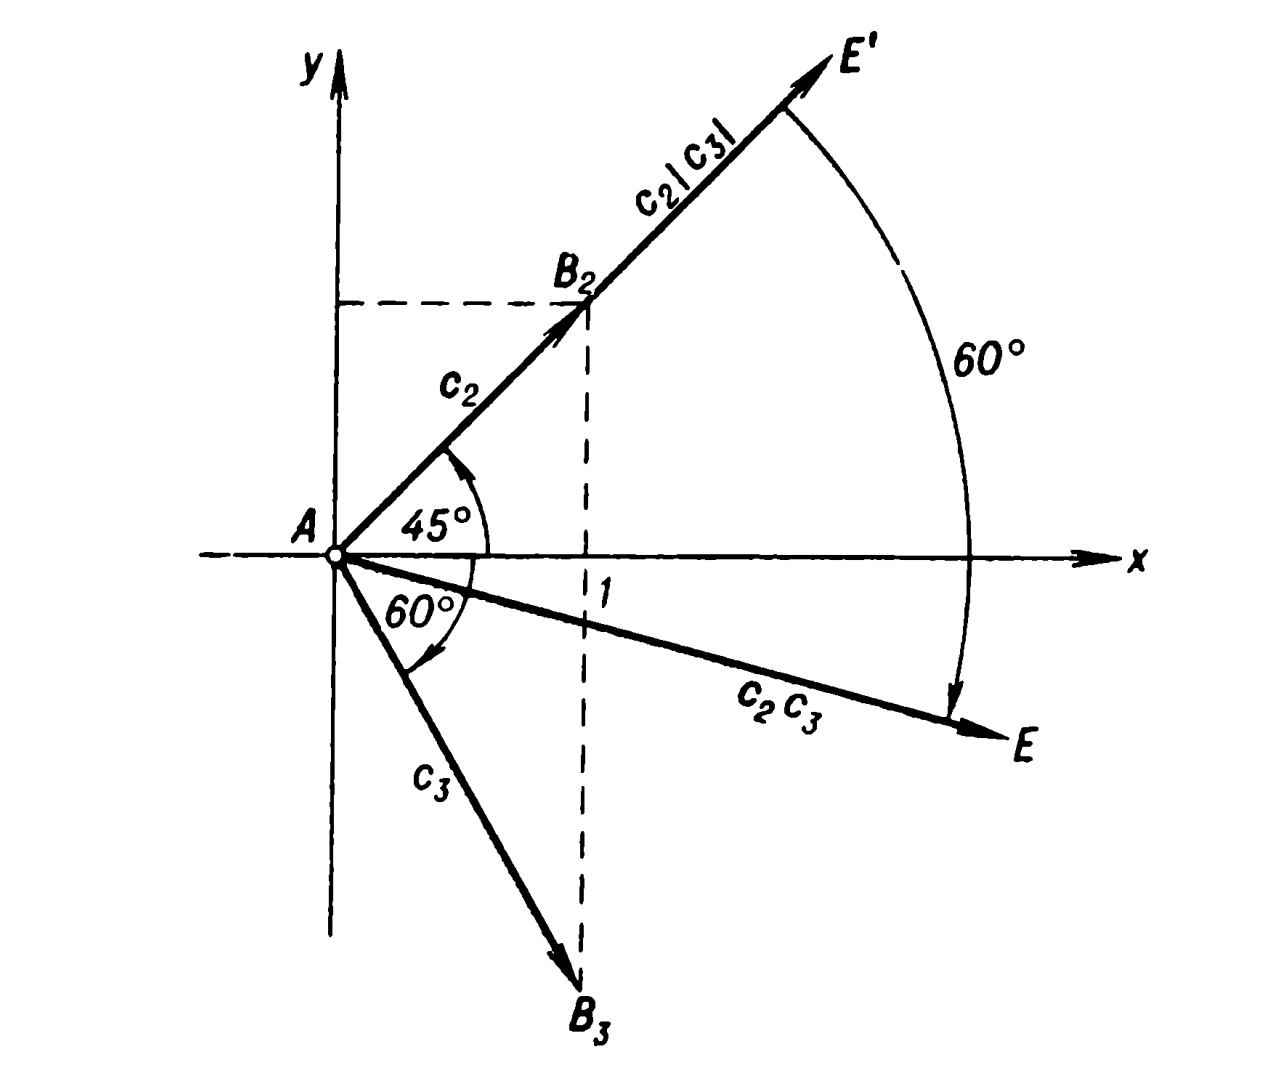
\includegraphics[width=.3\textwidth]{c1xc2} 
\end{center}
\end{figure}
%%%-----------------------------------------------------------------------------
Here is the multiplication of two vectors: $\langle 3,4\rangle$ and $\langle 5,12\rangle$ to produce the vector $\langle -33,56\rangle$. Note: $\langle 33,56,65\rangle$ is a Pythagorian triple.
\begin{figure}[h]
\begin{center}
\caption{Another Geometric Interpretation of Complex Number Multiplication (Drawn to Scale using Geogebra)}
\label{fig:complexmult2}
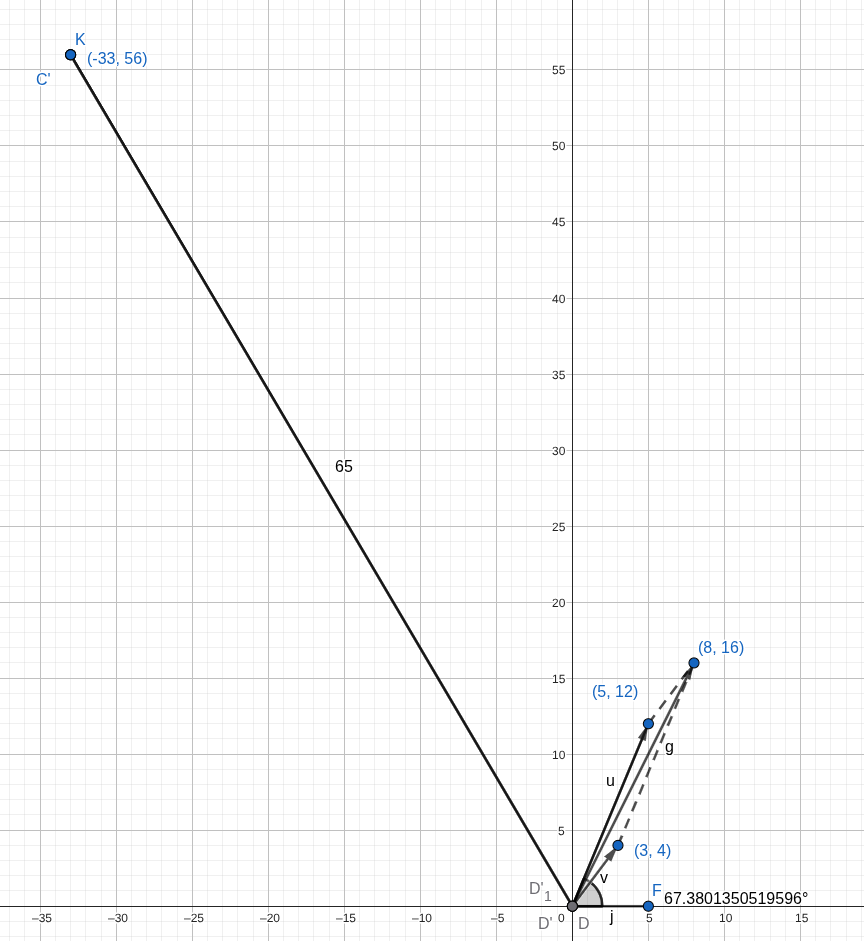
\includegraphics[width=.5\textwidth]{c1xc2-2} 
\end{center}
\end{figure}

\begin{problem}
\label{pr:affine}
If an operation for the ordered pairs of real numbers, denoted by $\boxdot$ again, is defined by
$$
\langle a,b\rangle\boxdot\langle c,d\rangle=\langle ac,ad+b\rangle
$$
, is it commutative? Is it associative?

Note: Looking strange is not necessarily a sign of being artificial or useless.
\end{problem}

\textbf{Solution}.

\begin{align*}
\langle a,b\rangle\boxdot\langle c,d\rangle=\langle ac,ad+b\rangle
\end{align*}
\begin{align*}
\langle c,d\rangle\boxdot\langle a,b\rangle=\langle ca,cb+d\rangle
\end{align*}

$\therefore \boxdot$ is not commutative in general; only commutative if $\frac{a-1}{b}=\frac{c-1}{d}$.
\begin{align*}
(\langle a,b\rangle\boxdot\langle c,d\rangle)\boxdot\langle m, n\rangle
&=\langle ac, ad+b\rangle\boxdot\langle m,n\rangle\\
&=\langle acm,acn+ad+b\rangle\\
\end{align*}
and
\begin{align*}
\langle a,b\rangle\boxdot(\langle c,d\rangle\boxdot\langle m, n\rangle)
&=\langle a,b\rangle\boxdot\langle cm,cn+d\rangle\\
&=\langle acm,acn+ad+b\rangle\\
\end{align*}

$\therefore \boxdot$ is associative.

\qedsymbol

\textbf{Halmos's Solution}.

Halmos describes an operation on functions: their composition. Consider two linear transformations of a real number (mapping of a real number onto another by a function $\mathbb {R}:\mathbb {R}$), $x$, where $a,b,c,d$ are known constants:
\begin{equation}
\!
\begin{aligned}
f(x)=ax+b \\
g(x)=cx+d
\end{aligned}\label{eq:fg}
\end{equation}

Then, is composition of functions commutative? 

$$
(f\circ g)(x)=f(g(x))=f(cx+d)=a(cx+d)+b=acx+ad+b
$$
and
$$
(g\circ f)(x)=g(f(x))=g(ax+b)=c(ax+b)+d=acx+bc+d
$$

$\therefore (f\circ g)\ne(g\circ f)$.

However, consider the application of $(f\circ g)$ to $x$. It yields a result that is the same as the affine transformation of $x$ by $(ac, ad+b)$ which is itself an affine transformation ($\boxdot$) of $\langle a,b\rangle$ and $\langle c,d\rangle$. And since $(f\circ g\circ h)=f\circ(g\circ h)=(f\circ g)\circ h$\footnote{That is, function composition is associative (which can be easily proved)}, $\boxdot$ is also associative. 

\qedsymbol

\begin{problem}
\label{pr:matrixmult}
If an operation for the ordered quadruples of real numbers, denoted by $\boxdot$, is defined by
$$
\langle a,b,c,d\rangle\boxdot\langle a',b',c',d'\rangle=\langle aa'+bc',ab'+bd',ca'+dc',cb'+dd'\rangle
$$
, is it commutative? Is it associative?
\end{problem}

\textbf{Solution}.
Since the multiplication of real numbers is commutative ($aa'+bc'=a'a+c'b$, and so on), the \textit{matrix multiplication} defined here is commutative.

The visual symmetry in this operation feels useful in proving its associativity, although one should carry out the operation rigorously to believe that it is associative. That is left out here (we wouldn't say ``as an exercise to the reader!'').

It's easier to visualize this as a matrix:

\[
  \begin{pmatrix}
    a & b\\
    c & d\\
  \end{pmatrix}
  \begin{pmatrix}
    a' & b'\\
    c' & d'\\
  \end{pmatrix}
  =
  \begin{pmatrix}
    aa'+bc' & ab'+bd'\\
    ca'+dc' & cb'+dd'\\
  \end{pmatrix}
\]

\qedsymbol

How is Problem [\ref{pr:affine}] a ``special case'' of Problem [\ref{pr:matrixmult}]?

Consider
\[
  \begin{pmatrix}
    a & b\\
    0 & 1\\
  \end{pmatrix}
  \begin{pmatrix}
    a' & b'\\
    0 & 1\\
  \end{pmatrix}
  =
  \begin{pmatrix}
    aa' & ab'+b\\
    0 & 1\\
  \end{pmatrix}
\]

The first row of the result is the affine tranform of the first rows of the two matrices on the left-hand side. Halmos, being an algebraist, does not describe it so, however. 

Also, is Problem [\ref{pr:affine}] a ``special case'' of Problem [\ref{pr:complexmult}]?
Consider
\[
  \begin{pmatrix}
    a & b\\
    -b & a\\
  \end{pmatrix}
  \begin{pmatrix}
    c & d\\
    -d & c\\
  \end{pmatrix}
  =
  \begin{pmatrix}
    ac-bd & ad+bc\\
    -bc-ad &-bd+ac\\
  \end{pmatrix}
\]
I still don't understand how matrix multiplication is a "more general" case of vector multiplication or affine transform; it might become clear later.

\begin{problem}
\label{pr:modularmult}
Is multiplication modulo 6 commutative? Is it associative? What if 6 is replaced with 7: do the conclusions for 6 remain true or do they change?
\end{problem}

\textbf{Solution}.
I should refresh my number theory, but I will defer that for now. Let me attempt my solution from first principles.

Since multiplication of integers is commutative ($ab=ba \forall a,b\in\mathbb{N}$), $ab\mod 6=ba\mod 6$. This is true when modulus is any positive integer.

Consider four integers, $a,b,c,M\mid M\ne 0$. We call $M$ the modulus. Then, according to the division algorithm, following integers, $q_1,r_1,q_2,r_2,q_3,r_3\mid r_1,r_2,r_3<M$ exist:
\begin{equation}
\!
\begin{aligned}
a &= Mq_1+r_1\\
b &= Mq_2+r_2\\
c &= Mq_3+r_3\\
\end{aligned}\label{eq:abcM}
\end{equation}

Then, $abc\mod M=r_1r_2r_3\mod M$, because it follows from Equation [\ref{eq:abcM}] that $abc\equiv r_1r_2r_3 \pmod{M}$.

Since the product of the integers, $r_1r_2r_3$, is associative, the modular multiplication operation, $abc\mod M$, is also associative.

\qedsymbol

\textbf{Halmos's Solution}.

Halmos warns that the most tedius way of solving this problem (or perhaps any problem) is by exhaustion: Prove something by examining it for every possibility. Thus, if there are only 6 integers (0 through 5) for which to prove commutativity and associativity of the modulo-6 multiplication, we can exhaust all the 36 ordered pairs and 216 ordered triples respectively, and we are done. That is clearly boring.

He provides another way that is equivalent to my approach (that uses the versatile division algorithm). I like my solution better!

However, he concludes his solution thus that makes us curious:
\begin{reflection}
An important difference between the modular arithmetic of 6 and 7 will
become visible later, but for most of the theory they act the same way, and that
is true, in particular, as far as commutativity and associativity are concerned.
\end{reflection}


\begin{problem}
\label{pr:smallsets}
\end{problem}
Problem [\ref{pr:modularmult}] shows that interesting operations can exist on small sets. In that problem we were working with (binary) operations whose results were members of a set: $S=\{0,1,2,3,4,5\}$ and whose operands any natural numbers. Although ``small sets'' like $S$ may sometimes be misleading, they may be useful to develop insight.

Problem [\ref{pr:2a2b}] asked about a binary operation (on real numbers) that was commutative but not associative ($a\boxplus b=2a+2b$).

Remarkably, the modulo 3 multiplication and the modulo 3 addition on any two numbers from $\{0,1,2\}$ are commutative \textit{and} associative:

\begin{table}[h!]
\centering
\begin{tabular}{l|ccc}
$\times$&0&1&2\\
\hline
0&0&0&0\\
1&0&1&2\\
2&0&2&1\\
\end{tabular}
\quad\quad\quad
\begin{tabular}{l|ccc}
+&0&1&2\\
\hline
0&0&1&2\\
1&1&2&0\\
2&2&0&1\\
\end{tabular}
\caption{Two commutative and associative operations}
\label{tab:twoops}
\end{table}

Is there an operation in a set of three elements that is commutative but not associative?

\textbf{Solution}.

Halmos hasn't defined what an ``operation \textit{in} a set of three elements'' means. For instance, is the operation on two members of a three-member set that returns a result which is also a member of the same set, or must the result of that operation (like the modular multiplication of Problem [\ref{pr:modularmult}]) on any two natural numbers be a member of that set?\footnote{Later on, when I was discussing this with my son, he spontaneously said, ``That means the set is \emph{closed} under that operation''} From context, I assume the former and restate the problem:

Is there a binary operation that is commutative but not associative that takes (two) elements of a three-member set and whose result is also a member of that set?\footnote{More technically: Is there a commutative but not associative operation on a 3-element set which is closed under that operation?}

How do we start solving such a problem? It \emph{feels} insurmountable. As I write this, I have no clear idea. ``C’est la vie'', I guess! However, we can try gathering facts and look for any patterns, connections, etc. We need to find a set of three numbers, three nonnegative integers, $S=\{a,b,c\}$ and define an operation $\openbox$ such that
\begin{enumerate}
\item The result of $\square$ on any two elements of $S$--$a,b$ for instance--is an element of $S$,
\item $\square$ is commutative, i.e., $a\square b= b\square a$, and
\item $\square$ is \emph{not} associative, i.e.,$a\square(b\square c)\ne (a\square b)\square c$
\end{enumerate}

This is what abstract algebra comprises. It wants us to focus on operations on entities more than the entities themselves; \emph{operations} are of essence.

A weird operation \emph{occurred} to me. Let's call it an \emph{exclude} operation, denoted by $\openbox$. Here is its definition for operands from any set $S$ that has three or more elements:

\begin{definition}[Exclude operation:$\openbox$]
It accepts two operands and returns an element from $S$ \emph{excluding} its operands. When more than one element is available, it returns the smallest (which is guaranteed to be unique).
\end{definition}

\begin{table}[h!]
\centering
\begin{tabular}{l|ccc}
$\downarrow x\openbox y\rightarrow$&2&3&5\\
\hline
2&3&{\textcolor{red}5}&{\textcolor{blue}3}\\
3&{\textcolor{red}5}&2&{\textcolor{LimeGreen}2}\\
5&{\textcolor{blue}3}&{\textcolor{LimeGreen}2}&2\\
\end{tabular}
\caption{$\openbox$ is commutative for $S=\{2,3,5\}$}
\label{tab:exclude}
\end{table}

Table [\ref{tab:exclude}] shows that $\openbox$ is commutative.

What about its associativity? 

$2\openbox(3\openbox 5)=2\openbox 2=3$, but $(2\openbox 3)\openbox 5=5\openbox 5=2$.

Since the two are not the same, $\openbox$ is not associative.

\qedsymbol

\begin{reflection}
$\openbox$ satisfies the problem's requirements, but I don't know why it works; its discovery feels like art. It is hard to say if I could have found it by deduction alone. 
\end{reflection}
\textbf{Halmos's Solution}.

The answer may or may not be easy to guess, but once it's correctly guessed it's easy to prove. The answer is yes, and anyone who believes that and sets out to construct an example is bound to succeed.

Call the three elements for which multiplication is to be defined $\alpha,\beta,\gamma$; the problem is to construct a multiplication table that is commutative but not associative. (Note: It's not clear why he wants to construct a ``multiplication table''. Perhaps he means `matrix'. So, what does a commutative-but-not-associative matrix look like?)

Question: what does commutativity say about the table? Answer: symmetry about the principal diagonal (top left to bottom right). That is: if the entry in row $\alpha$ and column $\beta$ is, say, $\gamma$, then the entry in row $\beta$ and column $\alpha$ must also be $\gamma$.

How can associativity be avoided? How, for instance, can it be guaranteed that $ (\alpha\times\beta)\times\gamma\ne\alpha\times(\beta\times\gamma)$?
\begin{reflection}
I stumbled at this question. Predicting whether a binary operation is commutative given its `matrix' is not that difficult. You check if the element $M_{ab}$ equals $M_{ba}$ ($a$ and $b$ respectively denote the row number and the column number).

What is the `matrix-test' of an associative binary operation? Looking only at the matrix (like the one in Table [\ref{tab:exclude}]) of some unknown binary operation, can one tell if it is associative? How? The two operations in Table [\ref{tab:twoops}] are too disparate to discern a common pattern for an associative operation!

Since associativity requires three operands, should I visualize a cube? However, the set is closed under this operation, so just looking at the matrix should be enough. 

Should I consider cases?

Time to peek at Halmos's discussion further in a way suggested by R. L. Moore \cite{Moore1966} (one line or two at a time, while considering this act a failure of sorts)?
\end{reflection}

Possible approach: make $\alpha\times\beta=\gamma$ and $\beta\times\gamma=\alpha$; then the associative law will surely fail if $\gamma\times\gamma$ and $\alpha\times\alpha$ are different. That's easy enough to achieve and the following table is one way to do it:

\begin{table}[h!]
\centering
\begin{tabular}{l|ccc}
$\times$&$\alpha$&$\beta$&$\gamma$\\
\hline
$\alpha$&$\alpha$&$\gamma$&$\beta$\\
$\beta$&$\gamma$&$\beta$&$\alpha$\\
$\gamma$&$\beta$&$\alpha$&$\gamma$\\
\end{tabular}
\caption{A commutative and not associative operation}
\label{tab:comnotassoc}
\end{table}
Here, for what it's worth, is a verbal description of this multiplication: the product of two distinct factors is the third element of the set, and the product of any element with itself is that element again.

\begin{reflection}
This is close to my exclude operation, but Halmos's explanation uses a neat trick. By making $\alpha\times\alpha$ not agree with $\gamma\times\gamma$, we can avoid associativity. However, does it mean that the associativity test is not as obvious as the commutativity test?
\end{reflection}

The sum of $0$ and any real number $\alpha$ is $\alpha$ again; the product of $1$ and any real number $\alpha$ is $\alpha$ again: $1\times\alpha=\alpha\times 1=\alpha$. This phenomenon is described by saying that $0,1$ are \textbf{identity element}s (or zero elements, unit elements, or neutral elements) of addition and multiplication respectively. 

\begin{reflection}
Commutativity appears a prerequisite for identity. An operation that is not commutative does not have an identity element. For instance, $a\div 1=a\ne 1\div a$. Therefore, the $\div$ operation on reals does not have an identity element.
\end{reflection}

\begin{reflection}
Identity elements of operations remind me of ``fixed points'' of functions.
\end{reflection}

\begin{problem}
\label{pr:idelem}
Which of the operations
\begin{enumerate}
\item double addition (Problem [\ref{pr:2a2b}]),
\item half double addition (Problem [\ref{pr:2ab}]),
\item exponentiation (Problem [\ref{pr:atob}]),
\item complex multiplication (Problem [\ref{pr:complexmult}]),
\item multiplication of affine transformations (Problem [\ref{pr:affine}]),
\item matrix multiplication (Problem [\ref{pr:matrixmult}]), and
\item modular addition and multiplication (Problem [\ref{pr:modularmult}])
\end{enumerate}
have an identity element?
\end{problem}
\textbf{Solution}.

Based on the definition of identity element above, we designate the \emph{constant} $a\in\mathbb{C}$ an identity element of the operation $\openbox$, if for some $b\in\mathbb{C}$, $a\openbox b$ equals $b$. We consider the set of complex numbers which may be thought bigger than that of real numbers. We apply this in turn for each item above. Of course, the other rules of arithmetic (and complex numbers) hold. This scheme feels straightforward.
\begin{enumerate}
\item For the double addition $\openbox$, by definition,
$$
a\openbox b=2a+2b
$$
For the prospective \emph{identity element} $a$ of the $\openbox$ operation, $a\openbox b$ equals $b$.
$$
b=2a+2b
$$
$$
\therefore a=-\frac{b}{2}
$$

Since $b$ can be any real number, $a$ must be so too. It cannot be a constant. That is a contradiction. Therefore, this operation does not have an identity element.
\item For the half double addition $\openbox$, by definition,
$$
a\openbox b=2a+b
$$
For the prospective \emph{identity element} $a$ of the $\openbox$ operation, $a\openbox b$ equals $b$.
$$
b=2a+b
$$
$$
\therefore 2a=0\implies a=0
$$
Therefore, $0$ is the identity element of the half double addition. 
\item For exponentiation, $b^a=b=b^1\implies a=1$. Therefore, $1$ is the identity element of exponentiation (like multiplication).
\item Complex multiplication is a bit more complicated. We are seeking a \emph{complex number} $c_1$, which is a pair of real numbers, $(a,b)$, such that $c_1\times c_2$ equals $c_2$, where $c_2$ is a pair of real numbers, $(c,d)$.

By definition,
$$
(a,b)\times(c,d)=(ac-bd,ad+bc)=(c,d)
$$
\begin{equation}
\label{eq:c1}
ac-bd=c
\end{equation}
and
\begin{equation}
\label{eq:c2}
ad+bc=d
\end{equation}

Equation [\ref{eq:c1}]$\times c+$Equation [\ref{eq:c2}]$\times d$ yields

$$
a(c^2+d^2)=c^2+d^2
$$
and, since $c^2+d^2\ne 0$, $a=1$. Then, from equation [\ref{eq:c1}], $bd=0\implies b=0$.

Therefore, the \emph{complex number} $(1,0)$ is the identity element of complex multiplication. Indeed, $(1,0)\times(c,d)=(1\times c-0\times d,1\times d+0\times c)=(c,d)$.

\item\label{item:affine} Affine transformation of two pairs of real numbers, $\langle a,b\rangle$ and $\langle c,d\rangle$, is the pair $\langle ac,ad+b\rangle$ for which to be the same as $\langle c,d\rangle$, $\langle a,b\rangle$ must be $\langle 1,0\rangle$, which is the identity element of affine transformation multiplication.
\item It's not hard to see that the matrix
\[
  \begin{pmatrix}
    1 & 0\\
    0 & 1\\
  \end{pmatrix}
\] 
is the identity element of matrix multiplication.
\item Since $0$ is the identity element of addition, it is also the identity element of modular addition. Similarly, since $1$ is the identity element of multiplication, it is also the identity element of modular multiplication. 
\end{enumerate}

\qedsymbol

A tradition followed in this book is that multiplication is a more general operation than addition. However, we should bear in mind addition is always commutative, multiplication may not be (e.g., matrix multiplication). 

\begin{reflection}
If addition is a ``special case'' of multiplication, exactly what makes the former commutative and latter not always so?

I hope that becomes clear in the due course \dots.
\end{reflection}

A mini-theorem now.
\begin{mini-theorem}
An operation (a binary operation) can have at most one identity element.
\end{mini-theorem}
\begin{proof}
We prove by contradiction that if an identity element exists for a given operation, it must be unique. Let there be two distinct identity elements, $e$ and $e'$. Thus, we assume that $e\ne e'$.

By definition, identity element(s) are commutative: $a\openbox b=b\openbox a$. If we use $a=e$ and $b=e'$, we get $e\openbox e'=e'\openbox e$ and it follows that $e=e'$. A contradiction. Therefore, $\openbox$ can have at most one identity element.
\end{proof}

Associativity and identity element of an operation are closely related to another interesting property of an operation defined below.

\begin{definition}[$*$ Inverse of $x$] 
Suppose that a binary operation $*$ has an identity element $\varepsilon$ such that $\varepsilon*x=x*\varepsilon=x\forall x$. Then, an element $\beta$ is called the ``$*$ inverse'' of $x$ if 
$$
x*\beta=\beta*x=\varepsilon
$$
\end{definition}

Note that an operation $*$ can have an identity element, but not every element in the set to which its operands belong has a $*$ inverse.
\begin{example} For the set $\mathbb{R}$ of real numbers, the multiplication operation $\times$ has an identity element $\varepsilon=1$; but $0\in\mathbb{R}$ does not have a $\times$ inverse. There is no $\beta\in\mathbb{R}$ such that $0\times\beta=1$. In other words, $0$ is the only real number that fails to be \emph{invertible} under $\times$. 
\end{example}
\begin{example} For the set $\mathbb{R}$ of real numbers, the addition operation $+$ has an identity element $\varepsilon=0$. Every real number has a $+$ inverse.
\end{example}
\begin{mini-theorem}
If $*$ is an associative operation, then any element it operates on has at most one inverse.
\end{mini-theorem}
\begin{proof}
Left as an exercise.
\end{proof}

\begin{problem}
\label{pr:complexinv}
For complex multiplication (defined in Problem [\ref{pr:complexmult}]), which ordered pairs $\langle a,b\rangle$ are invertible? Is there an explicit formula for the inverses of the ones that are?
\end{problem}

\textbf{Solution}.

\begin{reflection}
This felt like a straightforward problem. By extension of the real multiplication, perhaps $\langle 0,0\rangle$ is the only complex number whose (complex) inverse does not exist.
\end{reflection}

We want to learn something about the \emph{complex inverse} of $\langle a,b\rangle$. Let $\langle c,d\rangle$ be that inverse. Then, by definition,

$$
\langle a,b\rangle\cdot\langle c,d\rangle=\varepsilon=\langle 1,0\rangle
$$

It follows that 
$$
\langle ac-bd,ad+bc\rangle=\langle1,0\rangle
$$
And
\begin{equation}
\!
\begin{aligned}
ac-bd=1 \\
ad+bc=0
\end{aligned}\label{eq:complexinv1}
\end{equation}
Then after eliminating $d$, we get
\begin{equation}
\!
\begin{aligned}
c=\frac{a}{a^2+b^2} \\
d=\frac{-b}{a^2+b^2}
\end{aligned}\label{eq:complexinvformula}
\end{equation}

Therefore, if ${a^2+b^2}\ne 0$, a complex inverse of $\langle a,b\rangle$ exists. We can use the formula in equation [\ref{eq:complexinvformula}] to calculate the $\cdot$ inverse of any complex number. The only exception is the complex number $\langle 0,0\rangle$ whose $\cdot$ inverse does not exist because $a^2+b^2=0$.

\qedsymbol

\begin{problem}
\label{pr:affineinv}
For the multiplication of affine transformations (defined in Problem [\ref{pr:affine}]), which ordered pairs $\langle a,b\rangle$ are invertible? Is there an explicit formula for the inverses of the ones that are?
\end{problem}

\textbf{Solution}.
\begin{reflection}
This feels like an \emph{exercise}. Should I look at it like what P\'{o}lya said (It is better to solve a problem 5 different ways rather than solving five different problems the same way)?
\end{reflection}
Proceeding as above and using $\langle 1,0\rangle$ as the identity element of affine transformations (Cf. item [\ref{item:affine}]), it follows that

$$
\langle ac,ad+b\rangle=\langle 1,0\rangle
$$
$$
\therefore c=\frac{1}{a}, d=-\frac{b}{a}
$$

The affine inverse of $\langle a,b\rangle$ is $\langle\frac{1}{a},-\frac{b}{a}\rangle$ which exists if $a\ne 0$.

\textbf{Halmos's Solution}.

Halmos proceeds along similar lines. However, he draws our attention to the fact that affine transformation is not commutative! 

\begin{reflection}
That's strange! Commutativity is a requirement for the definition of the identity element of an operation. If affine transformation is not commutative, how can its inverse (even the so-called `right' inverse) be defined?
\end{reflection}

%%%-----------------------------------------------------------------------------
\MakeBibliography[nosplit]
%%%-----------------------------------------------------------------------------

%%%-----------------------------------------------------------------------------
\end{document}
%%%-----------------------------------------------------------------------------
